\chapter{Modellistica Matematica}\label{ch:math}

\begin{flushright}
\textit{``Grazie al modello matematico posso dirvi\\ Come è nato l'universo. Non il Perché.''}
\end{flushright}
\begin{flushright} \textsc{Stephen Hawking} (1942 - vivente) \end{flushright} 
\begin{flushright} { } \end{flushright}

Nella descrizione di una gran parte di fenomeni nelle scienze applicate si fa uso di modelli matematici. Le scienze applicate non sono solo quelle classiche; oltre alla fisica e alla chimica, la modellistica matematica è entrata pesantemente in discipline complesse come la finanza, la biologia, la medicina. Per ``modello'' intendiamo un insieme di equazioni in grado di catturare le caratteristiche della situazione in esame e poi di descriverne, prevederne e controllarne lo sviluppo.

Un modello matematico è in generale costruito a partire da due mattoni principali \cite{salsa}: \textit{leggi generali} e \textit{relazioni costitutive}. Le leggi generali sono quelle della chimica e della fisica e si presentano come leggi di conservazione o di bilancio (della massa, dell'energia, del momento \ldots). Le relazioni costitutive sono invece di natura sperimentale e dipendono dalle caratteristiche contingenti del fenomeno in esame. Ne sono esempi la legge di Fourier per il flusso di calore e quella di Fick per la diffusione di una sostanza o la legge di Ohm per la corrente elettrica. Il risultato della combinazione dei due mattoni è di solito un'equazione o un sistema di equazioni differenziali.	


\section{La scienza (e l'arte) della modellistica}

La modellistica matematica è un linguaggio usato per descrivere in maniera disambigua, concisa e consistente un dato fenomeno \cite{khoo}. Disambigua perché consente a differenti ricercatori di usare e testare lo stesso modello senza essere confusi riguardo alle ipotesi usate nel modello. Concisa perché le equazioni impiegate nel modello essendo basate, almeno in larga parte, su una conoscenza pregressa del fenomeno in esame, sono utili per archiviare in forma compatta tali informazioni. Infine la consistenza del modello deriva dalle regole operative proprie della matematica. Il rovescio della medaglia consiste nel fatto che le ipotesi insite nel modello sono, appunto, solo ipotesi. Esse rappresentano ciò che si ritiene essere alla base di un dato fenomeno, e spesso si tratta di ipotesi incorrette o troppo semplicistiche. Di conseguenza il comportamento del modello solitamente differisce dal comportamento della realtà che si vuole studiare. Ciononostante la potenza della modellistica matematica sta nell'uso del metodo scientifico: la discrepanza fra \textit{previsioni} e \textit{osservazioni} può essere usata come \textit{feedback} per stabilire l'inadeguatezza di una o più ipotesi. Ciò consente di tornare alla fase di sviluppo del modello, modificarne le ipotesi, e osservarne di nuovo il comportamento. Questo altalenarsi di \textit{deduzione} e \textit{abduzione}\footnote{la \textit{deduzione} è un tipo di ragionamento che opera mediante ipotesi esatte; è un ragionamento certo, nel senso che la conclusione segue necessariamente dalle ipotesi, ma non è informativo, non aggiunge nessuna nuova informazione a quella che già era implicita nelle ipotesi; l'\textit{abduzione} invece è un ragionamento col quale, date certe conclusioni, si tenta di trovare delle possibili ipotesi che le spieghino; non c'è garanzia che le ipotesi trovate siano quelle giuste, ma l'abduzione <<è l'unico tipo di ragionamento che genera una nuova idea>> ed è <<il primo passo del ragionamento scientifico>>. (C. S. Peirce. \textit{Opere}. Bompiani, 2003).} continua finché non si sia soddisfatti di ciò che il modello è in grado di spiegare definendolo, a questo punto, un ``buon'' modello. In seguito alla fase appena descritta, detta di \textit{validazione}, è possibile usare il modello per prevedere l'esito sperimentale di un fenomeno sotto condizioni non ancora indagate. Tali previsioni potranno servire da guida per la pianificazione e progettazione di futuri esperimenti.

\section{Ottimizzazione di un modello}\label{sec:simplex}
L'ottimizzazione è una parte integrante del processo di validazione. Consiste nello stimare, qualora non fossero già noti dalla letteratura o da precedenti ottimizzazioni, i parametri del modello in modo che questi minimizzino (o massimizzino) una qualche \textit{criterion function}\footnote{per \textit{criterion function} si intende una funzione $J:\mathbb{R}^n\rightarrow \mathbb{R}$, di solito quadratica, che prende in ingresso gli $n$ parametri da ottimizzare e dà in uscita un valore reale.} che indichi il grado di scarto (o corrispondenza) fra modello e realtà. La criterion function più usata è la somma degli scarti quadratici fra output reale e output del modello, cioè:
$$J = \sum_n\bigl(y(n)-y_{pred}(n)\bigr)^2 = \sum_n e(n)^2$$
Qui $n$ sono gli istanti temporali scelti per il calcolo dei valori; si tratta degli istanti di tempo in cui sono state effettuate le misure reali sul sistema fisiologico. Con la criterion function così definita l'obiettivo dell'ottimizzazione è trovare la combinazione dei valori dei parametri che la minimizzano. In figura \figurename~\ref{opt_scheme} è mostrato lo schema del processo di ottimizzazione. Bisogna notare che se il modello fornisse una descrizione accurata della dinamica del sistema fisiologico, allora gli errori residui $e(n)$ dovrebbero essere dello stesso ordine di grandezza degli errori di misura.
\begin{figure}[htb]
	\centering
	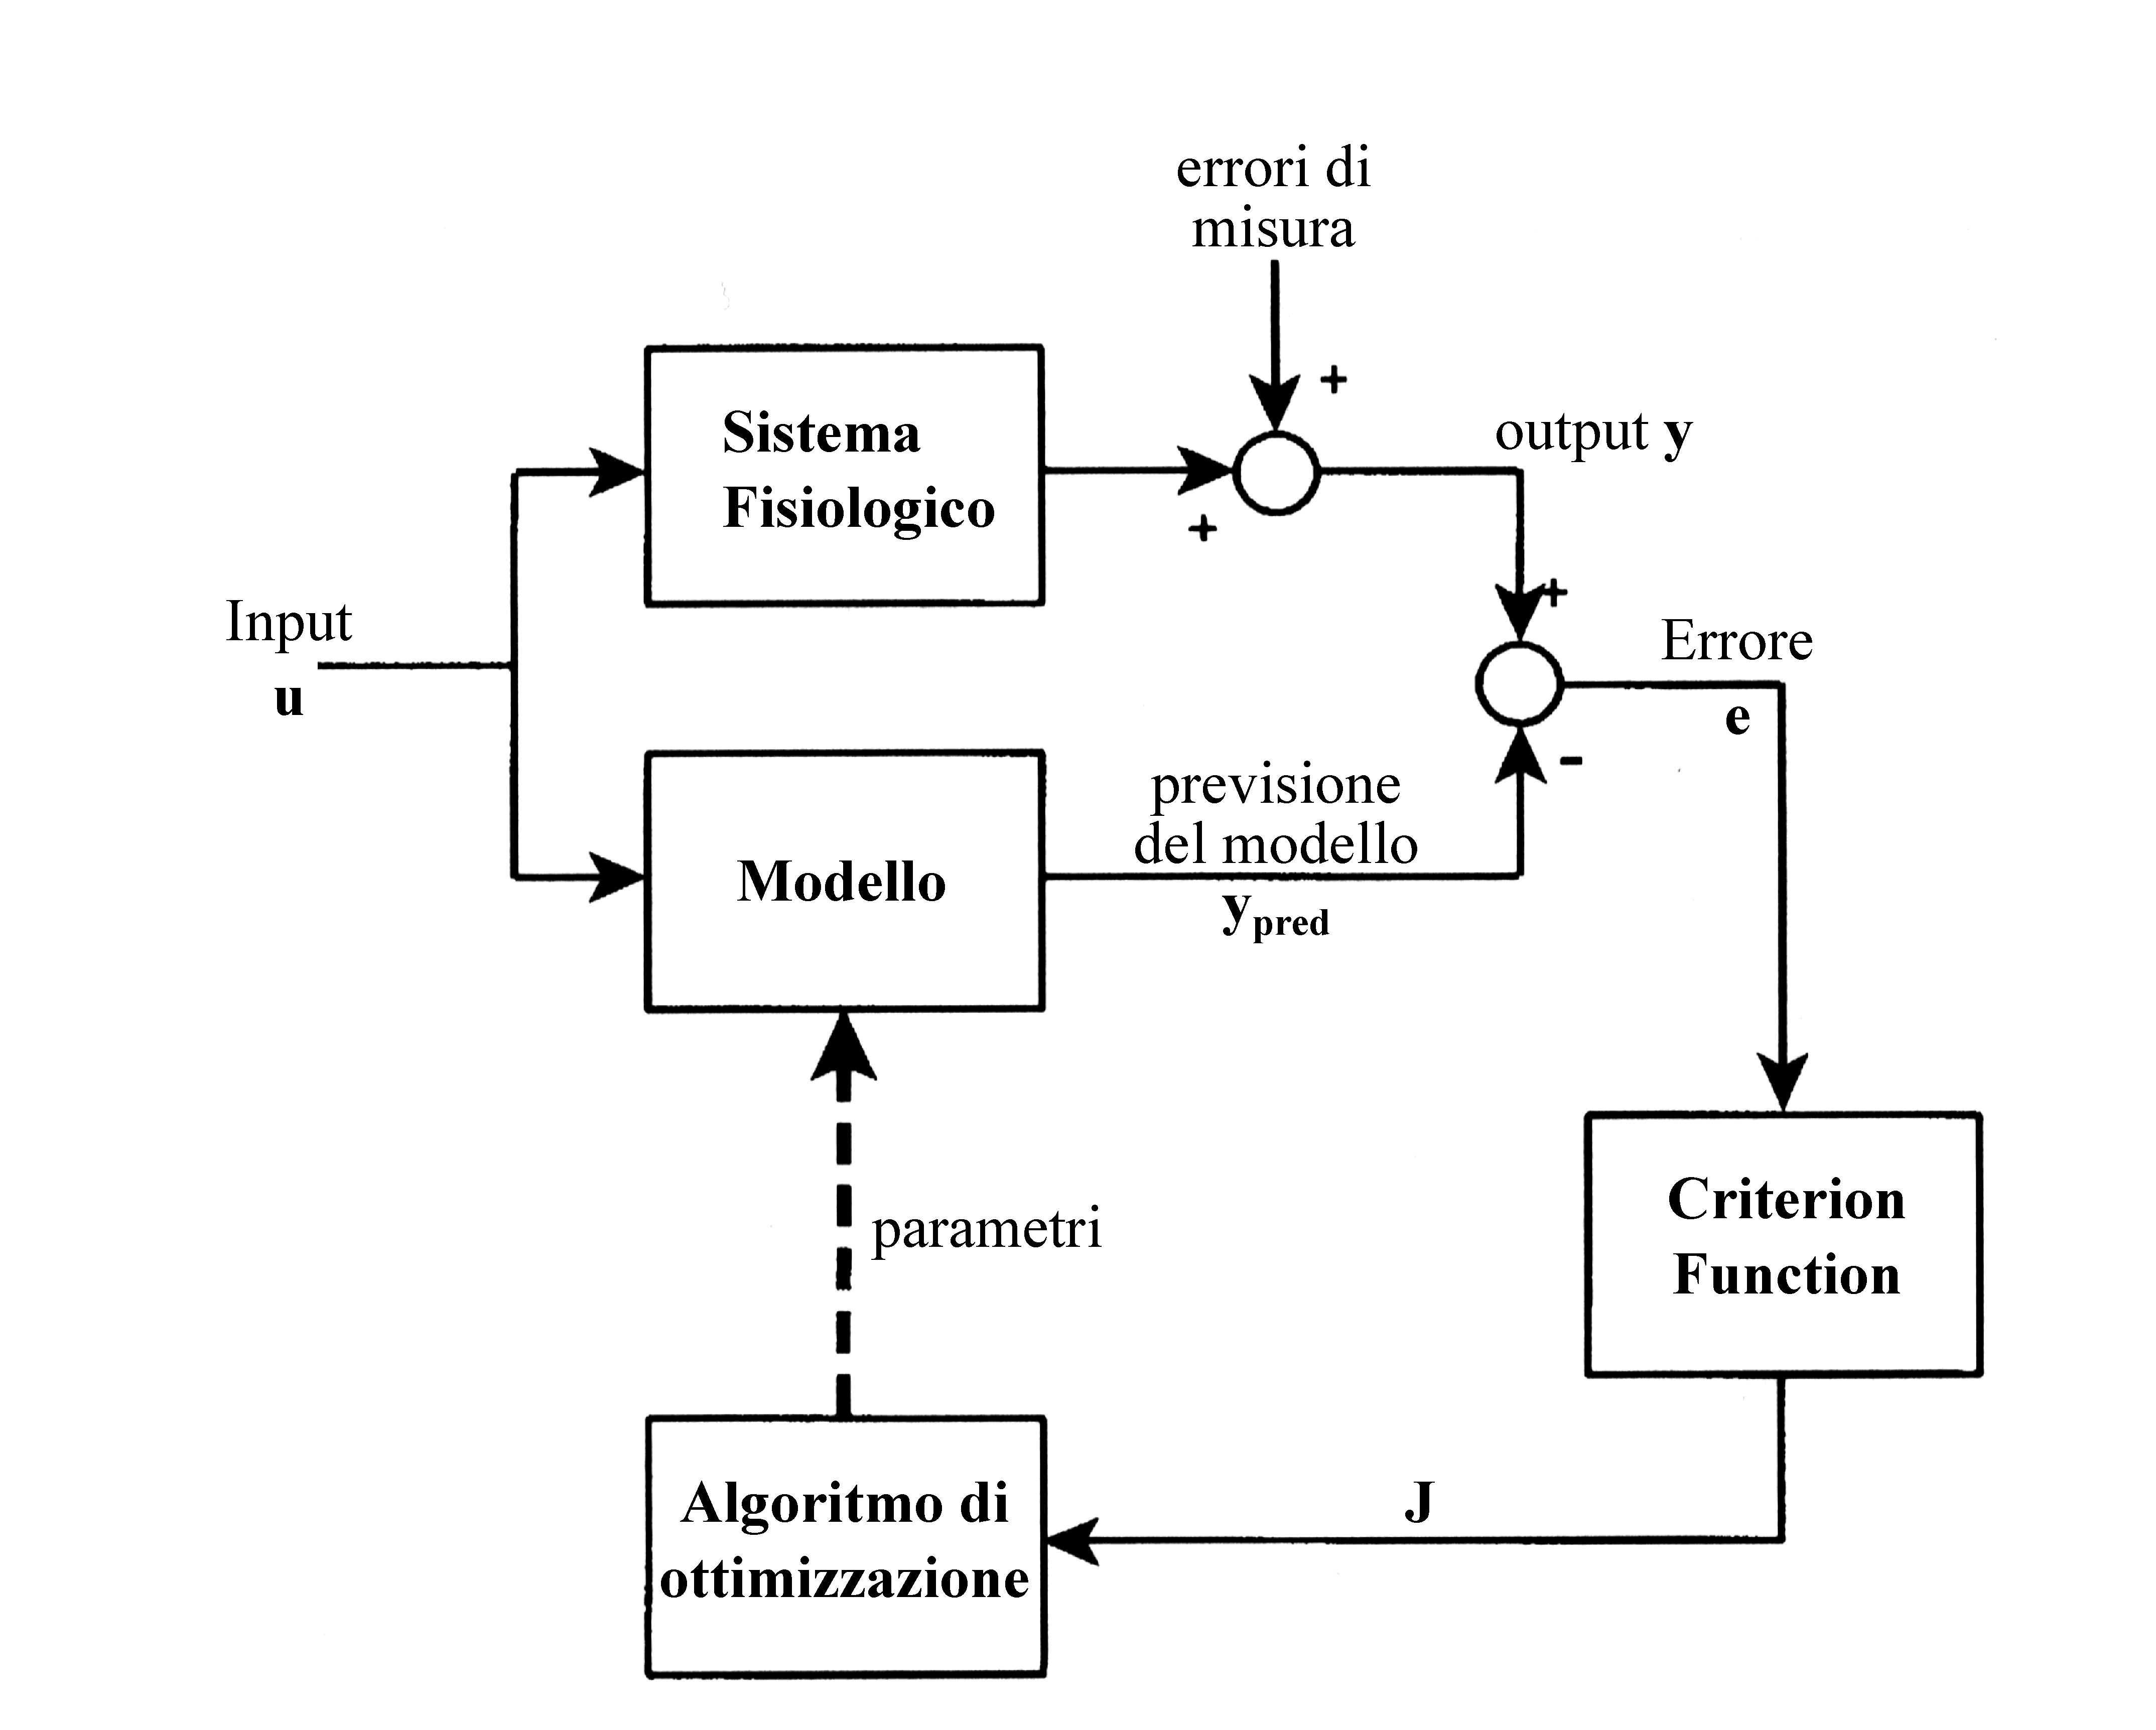
\includegraphics[width=0.82\textwidth]{immagini/opt_scheme.eps}
	\caption{Diagramma schematico del processo di ottimizzazione di un modello.}\label{opt_scheme}		
\end{figure}
Dopo quella della criterion function un'altra scelta importante è quella dell'algoritmo di ottimizzazione. La classe di algoritmi più comunemente usata è quella della \textit{discesa del gradiente}: ipotizzando di voler stimare due parametri, $J$ è una funzione dei parametri $\theta_1$ e $\theta_2$, e  il metodo del gradiente consiste nell'inizializzare i parametri con un valore arbitrario all'interno del loro range di validità, identificato dal punto $P$ nell spazio tridimensionale generato dagli assi cartesiani $\theta_1$, $\theta_2$ e $J$. Successivamente si calcola il gradiente di $J$ nel punto $P$ e ci si muove nella direzione discendente. La dimensione dello \textit{step} di discesa differisce a seconda del particolare metodo utilizzato.

I metodi del gradiente sono i più dispendiosi dal punto di vista computazionale perché, per ogni step iterativo, richiedono il calcolo delle derivate di $J$ rispetto ad ogni parametro; inoltre, nel caso in cui la superficie $J$ sia irregolare, tendono a restituire come risultato un falso minimo globale. Un'alternativa più efficiente, che non richiede alcun calcolo di derivate, è l'algoritmo del \textit{simplesso} di Nelder-Mead \cite{Nelder-Mead}. Per un problema a due parametri il simplesso prende la forma di un triangolo, mentre per un problema a tre parametri quella di un tetraedro. La funzione che in Matlab implementa il metodo del simplesso è \verb|fminsearch|. Con questa funzione non è però possibile stabilire dei limiti al dominio di ricerca dei parametri. Tali limiti sono indispensabili per contenere i parametri di riferimento all'interno di un range fisiologico accettabile. Per questo motivo si è scelto di usare la funzione \verb|fmincon|, che richiede come ingressi la criterion function da minimizzare, il punto di partenza e il dominio di ricerca del parametro da ottimizzare. Tale funzione, infatti, permette di risolvere problemi di ottimizzazione non lineare vincolata, utilizzando un metodo di programmazione quadratica sequenziale (SQP). Per informazioni più dettagliate si consulti la documentazione di Matlab.



